
%{{{ Preamble

\documentclass[journal,a4paper]{IEEEtran}
\hyphenation{op-tical net-works semi-conduc-tor}

%{{{ Packages

\usepackage[l2tabu,orthodox, abort]{nag}
\usepackage{fontspec}

\usepackage{microtype}
\frenchspacing

\usepackage{polyglossia}
\setdefaultlanguage{english}

\usepackage{graphicx}
\graphicspath{{../material/paper/}{../material/background/}}

\usepackage{minted}
\usepackage{lipsum}
\usepackage{url}
%}}}


%{{{ New commands

%\newcommand{\source}[1]{{\caption{\tiny {\fontspec{ProFontWindows} {Source: #1} } } } }
\newcommand{\source}[1]{Source: #1}
%}}}


%{{{ Avebritations

\def\krste/{Krste Asanovi\'c}
\def\CC/{C\nolinebreak\hspace{-.05em}\raisebox{.4ex}{\tiny\textbf{+}}\nolinebreak\hspace{-.03em}\raisebox{.4ex}{\tiny\textbf{+}}}
%}}}



%}}}



\addto\captionsenglish{%
  \renewcommand\tablename{Listing}%
  %\renewcommand{\figurename}{Fig.}%
  %\renewcommand{\contentsname}{Table of Contents}%
}



\begin{document}
%\setlength{\parindent}{0mm}

%{{{ Title, author, abstract and keywords

\title{RISC-V --- Architecture and Interfaces\\The RocketChip}


\author{Moritz~N\"oltner-Augustin\\%
University of Heidelberg, ZITI}
%	\IEEEcompsocitemizethanks{\IEEEcompsocthanksitem M. N\"oltner is enrolled at the University of Heidelberg and is currently pursuing a B.S. degree in applied informatics.\protect\\
%	E-mail: sh386@ix.urz.uni-heidelberg.de}%
%\thanks{Manuscript received January 6, 2015; revised January 12, 2015.}}%

% The paper headers
\markboth{Advanced Seminar ``Computer Engineering'', UNIVERSITY OF HEIDELBERG WT16/17}%
{Shell \MakeLowercase{\textit{et al.}}: RISC-V --- Architecture and Interfaces\\The RocketChip}

\maketitle

\begin{abstract}
	This paper gives a short overview of the RocketChip system-on-chip generator and how to use it.
\end{abstract}

% Note that keywords are not normally used for peerreview papers.
\begin{IEEEkeywords}
	RISC-V, RocketChip, Boom, SoC generator.
\end{IEEEkeywords}

%}}}

%{{{
\section{Introduction}
\IEEEPARstart{C}{omputer} technology has seen the rise and fall of many instruction set architectures (ISAs) over time.
Proprietary ISAs not only lead to fragmentation of the CPU market, but are also vulnerable to extinction when their proprietor companies run into financial troubles.
Along with design complexity and licensing issues, these considerations led \krste/ et al.\ to decide upon creating a new and free ISA for their next round of research projects at the University of California Berkeley (UCB).
This fifth reduced instruction set ISA developed at UCB, called RISC-V, is --unlike its predecessors-- not only meant for teaching but also actual implementation.
With three supported word-widths (32, 64 and 128 bits), RISC-V is aimed at all possible computational environments ranging from small embedded systems up to full scale supercomputers.
To facilitate widespread adoption, the ISA is licensed permissively, allowing use for academic and commercial use in open- and closed-source designs free of charge and now, roughly 4 years after its inception, RISC-V is used in a number of roles:

\begin{itemize}
	\item The LowRISC project aims to become the ``linux of the hardware word''
	\item SiFive and Open-V are creating custom silicon products
	\item ETH Zurich and Università di Bologna cooperate to create a state-of-the-art parallel microcontroller
	\item IIT Madras creates a processor
	\item NVIDIA will use the RISC-V ISA for the replacement of their Falcon processor
	\item UCB uses RISC-V processors for research purposes as well as for teaching
\end{itemize}
%}}}


%{{{
\section{RocketChip}
The UCB currently developes three lines of RISC-V processors, Sodor, Rocket and Boom.
Sodor is a collection of simple processors for use in lectures, Rocket is a scalar in-order processor for personal applications and Boom is a superscalar out-of-order processor for high performance applications.
All three are written in Chisel (Creating Hardware in a Scala Embedded Language), a hardware description language --as the name implies-- embedded in Scala.
Chisel allows compilation into three distinct target formats, the first of which is a cycle accurate \CC/ model for fast simulation and software development, the other targets are verilog code aimed at implementation in an FPGA or ASIC\@.
For Rocket and Boom there is a generator framework that can create a whole parametrised system around the processor cores, called RocketChip.
It will create one or more Rocket, Boom or custom cores, surround it with caches, optionally an FPU and accelerators to form one or more tiles. Then the tiles are connected to a TileLink network. The CPU is finished by adding TileLink to AXI4 converters to provide a well known bus interface to the outside world. Figure~\ref{rcov} shows a schematic of the generated system.

%{{{ RocketChip overview

\begin{figure}[!t]
	\centering
	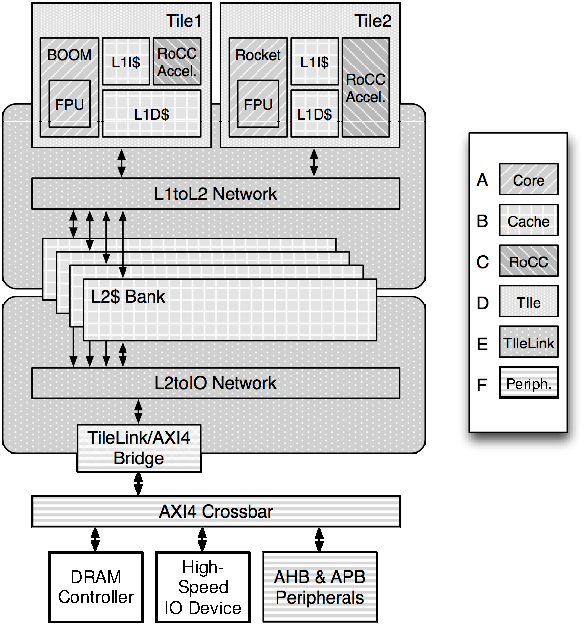
\includegraphics[width=3in]{rcov}
	\caption{Overview of the components of RocketChip.\newline\hspace{\linewidth}\source{Image taken from~\cite{rcgen}}.}
	\label{rcov}
\end{figure}
%}}}

\subsection{General Usage}
The RocketChip is maintained in a Git repository.
To build the default-configuration RocketChip, one only has to clone the repository, build the included GCC toolchain for RISC-V, and run ``\texttt{make}'' as shown in listing~\ref{rcclone}. For building a Boom-chip, the steps are identical except that one also has to checkout the ``\texttt{boom}'' branch of the same repository which then includes the Booms repo as a submodule.
%Listing~\ref{rcclone} shows the steps needed to build a RocketChip.

%{{{ RocketChip build steps /1

\begin{table}
	\caption{Downloading and initialising the Rocket chip repository.\newline\hspace{\linewidth}Source: Collected from~\cite{rc_github} and~\cite{boom_github}.}
	\label{rcclone}
	\begin{minted}[fontsize=\small, gobble=2, tabsize=2]{bash}
		# $RC is some place in the file system
		cd $RC
		git clone \
		https://github.com/ucb-bar/rocket-chip.git
		cd rocket-chip
		# If one wants to build a Boom
		#git checkout boom
		git submodule update --init --recursive
	\end{minted}
\end{table}
%}}}

If the environment variable RISCV is not set to point to a sane installation of the toolchain, the following build steps will fail, so the next part is building the RISCV-toolchain as shown in listing~\ref{rctoolchain}.

%{{{ RocketChip build steps /2

\begin{table}
	\caption{Building the RSCV-toolchain.\newline\hspace{\linewidth}Source: Collected from~\cite{rc_github} and~\cite{boom_github}.}
	\label{rctoolchain}
	\begin{minted}[fontsize=\small, gobble=2]{bash}
		cd $RC/riscv-tools
		export RISCV=/where/to/install/toolchain
		export PATH="${PATH}:$RISCV/bin"
		./build.sh # Takes about 45 min
	\end{minted}
\end{table}
%}}}


\subsection{Building a Configuration}
The makefile has a variable named ``\texttt{CONFIG}'' which is set to the name of a configuration.
A configuration is a set of configuration options that define the generated system.
%This configuration is the set of configuration options that define the generated system.
Available configuration options can be found in \texttt{\$(RC)/src/main/scala/coreplex/Configs.scala}, and include for example

%{{{ RocketChip config options

\begin{itemize}
	\item What core[s] (Rocket | BOOM | Custom)
	\item \#Tiles
	\item TileLink config
	\item Bootrom
	\item Debug hardware (\#Breakpoints, \#Performance Counters)
	\item What floating point unit
	\item What multiplication and division logic
	\item What atomic instructions
	\item Cache configuration (\#sets, \#ways, \#TLB entries, ECC, replacement policy)
\end{itemize}
%}}}
.
These options are grouped into different build configurations which can be found in \texttt{\$(RC)/src/main/scala/rocketchip/Configs.scala}.
Building one of the pre-defined configurations is as simple as setting the \texttt{CONFIG} variable while \texttt{make}-ing the project. Listing~\ref{rcmake} shows the steps to build the emulator and the verilog source code for a certain RocketChip configuration.

%{{{ RocketChip build steps /3

\begin{table}
	\caption{The build steps for creating a Rocket chip.\newline\hspace{\linewidth}Source: Collected from~\cite{rc_github} and~\cite{boom_github}.}
	\label{rcmake}
	\begin{minted}[fontsize=\small, gobble=2]{bash}
		cd $RC/emulator
		make run CONFIG=BOOMConfig
		make run CONFIG=ExampleSmallConfig
		cd $RC/vsim
		make -jN CONFIG=ExampleSmallConfig # about 20 min
	\end{minted}
\end{table}
%}}}


\subsection{Creating a Configuration}
To define a new configuration, a new child class of \texttt{Config} will have to be defined which contains the relevant configuration options. \texttt{\$RC/src/main/scala/coreplex/Configs.scala} contains those configurations.
%{{{ Config options

\begin{table}
	\caption{Extract of some configuration options found in \texttt{\$RC/src/main/scala/coreplex/Configs.scala}.}
	\label{config_options}
	\begin{minted}[fontsize=\small, gobble=2]{java}
		...
		case CacheBlockBytes => 64
		case CacheName("L1D") => CacheConfig(
		nSets= 64,
		nWays= 4,
		rowBits= site(L1toL2Config).beatBytes*8,
		nTLBEntries= 8,
		cacheIdBits= 0,
		splitMetadata = false)
		...
	\end{minted}
\end{table}
%}}}


%%{{{ Config
%
%\begin{table}
%	\caption{The build steps for creating a Rocket chip.\newline\hspace{\linewidth}Source: Collected from~\cite{rc_github} and~\cite{boom_github}.}
%	\label{rcmake}
%	\begin{minted}[fontsize=\small, gobble=2]{java}
%	\end{minted}
%\end{table}
%%}}}










%\lipsum





%}}}


%{{{
\section{Conclusion}
%Both \twi\ and SPI are very mature, while still up-to-date bus systems for low-speed, low-complexity interconnection of integrated circuits.
%With their wide acceptance and when used as intended, both \twi\ and SPI are recommendable and reliable bus systems.

%}}}

\bigskip
%\vfill

%{{{
\begin{thebibliography}{1}
	\bibitem{rcgen}
	Asanovi\'c, Krste/Avizienis, Rimas/Bachrach, Jonathan et at. (2016)\\
	The Rocket Chip Generator.\\
	Technical Report No. UCB/EECS--2016--17, EECS Department, University of California, Berkeley.\\
	\url{http://www2.eecs.berkeley.edu/Pubs/TechRpts/2016/EECS--2016--17.html}\\

	\bibitem{rc_github}
	The RocketChip github pages\\
	\url{https://github.com/ucb-bar/rocket-chip}\\
	\url{https://github.com/ucb-bar/project-template}\\

	\bibitem{boom_github}
	The Berkeley Out Of Order Machine github page\\
	\url{https://github.com/ucb-bar/riscv-boom}\\


\end{thebibliography}
\enlargethispage{-5in}
%}}}


\end{document}
